\begin{frame}
    \frametitle{Filtro de Partículas (Particle Filter)}
    \note{Información extraída de Vídeo de Cyrill Stachniss https://youtu.be/MsYlueVDLI0}
    \footnotesize
    \begin{itemize}
        \item Con EKF estamos restringidos a distribuciones Gaussianas.
        \item Cuando usamos EKF obtenemos una Distibuión Gaussiana que describe dónde se encuentra el robot.
        \item En Particle Filter utilizamos partículas o hipótesis que describen dónde podría estar el robot.
        \item En vez de tener una forma paramétrica como es EKF, que describimos la distribución de probabilidad con los parámetros media $\mu$ y covarianza $\covariance$. Partible Filter utiliza muestras no-paramétricas como hipótesis sobre dónde el robot podría estar.
    \end{itemize}
    
    
   	\begin{center}
        \movie[loop]{\includegraphics[width=0.4\columnwidth]{images/particle_filter/particle_filter_video.jpg}}{videos/particle_filter.mp4}
    \end{center}
    
    \note{Vídeo extraído de https://rse-lab.cs.washington.edu/projects/mcl/animations/global-floor.gif}
    
\end{frame}

\begin{frame}
    \frametitle{Aproximación de una Función}
    \note{Información extraída de Vídeo de Cyrill Stachniss https://youtu.be/MsYlueVDLI0}
    \footnotesize
    
    \begin{itemize}
        \item Objetivo: Poder estimar cualquier \textbf{distribución de probabilidad arbitraria}.
    \end{itemize}
    
    \begin{center}
    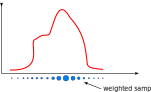
\includegraphics[width=0.5\columnwidth]{./images/particle_filter/arbitrary_distribution.pdf}
    \end{center}
    
\end{frame}

\begin{frame}
    \frametitle{Utilizando Muestras (Partículas)}
    \note{Información extraída de Vídeo de Cyrill Stachniss https://youtu.be/MsYlueVDLI0}
    \footnotesize
    \begin{itemize}
        \item \textbf{Múltiples muestras} para representar una distribución de probabilidad arbitraría
        \item Las muestras son están más agrupadas en algunas áreas en otras menos. La cantidad de partículas por unidad de área describe que tan probable es que el robot se encuentre en esa área.
        \item Cada muestra está acumulando un poco de ``masa de probabilidad''.
        \item Las muestra puede ser vista como una aproximación a la función de densidad de probabilidad (pdf).
        \item Para obtener la pdf, hay que integrar sobre una cierta área de manera de obtener la probabilidad matemática de que el robot se encuentre en dicha área.
    \end{itemize}
    
    \begin{center}
    \includegraphics[width=0.5\columnwidth]{./images/particle_filter/arbitrary_distribution_samples.pdf}
    \end{center}
    
\end{frame}

\begin{frame}
    \frametitle{Utilizando Muestras con Peso}
    \note{Información extraída de Vídeo de Cyrill Stachniss https://youtu.be/MsYlueVDLI0}
    \footnotesize
    \begin{itemize}
        \item \textbf{Múltiples muestras con peso} para representar una distribución de probabilidad arbitraría
        \item Es posible reducir el número de muestras que necesitamos, si le agregamos pesos a cada muestra
        \item Mientras más peso tiene una muestra, más masa de probabilidad hay en esa región
        \item Los pesos de todas las partículas juntas deben sumar 1
        \item Al inicio, podríamos agregarle a cada muestra un peso uniforme. Por ejemplo, si tenemos $n$ muestras, entonces cada muestra tiene peso $\frac{1}{n}$
    \end{itemize}
    
    \begin{center}
        \includegraphics[width=0.5\columnwidth]{./images/particle_filter/arbitrary_distribution_weighted_samples.pdf}
    \end{center}
    
\end{frame}

\begin{frame}
    \frametitle{Filtro de Partículas (Particle Filter)}
    \note{Información extraída de Vídeo de Cyrill Stachniss https://youtu.be/MsYlueVDLI0}
    
    \footnotesize
    \begin{itemize}
        \item Notar que es una aproximación de la pdf
        \item Es importante tener un número de muestras suficientes para poder representar la fdp adecuadamente.
    \end{itemize}
    
    
\end{frame}

\begin{frame}
    \frametitle{Conjunto de Partículas}
    
    \begin{itemize}
        \item Conjunto de partículas con peso
            
        \begin{center}
            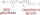
\includegraphics[width=0.5\columnwidth]{./images/particle_filter/weighted_samples.pdf}
        \end{center}

        \item Las partículas representan la posterior belief dada por
        \begin{equation*}
            p(x) = \sum_{j=1}^{J} w^{[j]} \delta_{x^{[j]}}(x)    
        \end{equation*}
        donde $\delta_{x^{[j]}}(x)$ es la función de Dirac centrada en la ubicación de la partícula $x^{[j]}$.

        \begin{equation*}
            \delta(y) = 
            \begin{cases} 
            \infty, & y = x^{[j]} \\ 
            0, & y \neq x^{[j]} 
            \end{cases};    
        \end{equation*}

        \note{La función tiende a infinito cuando $x=j$ y, para cualquier otro valor de $x$, es igual a 0.}

    \end{itemize}
   
\end{frame}


\begin{frame}
    \frametitle{Partículas para Aproximar}
    
    \begin{itemize}
        \item Partículas para aproximar una función
        
        \begin{center}
            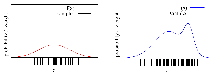
\includegraphics[width=0.8\columnwidth]{./images/particle_filter/particles_for_approximation.pdf}
        \end{center}

        \item Más partículas caen en una región, más alta es la probabilidad de la región
    \end{itemize}
    
    \begin{center}
        \alert{¿Cómo obtener dichas muestras?}
    \end{center}

\end{frame}

\begin{frame}
    \frametitle{Forma Cerrada de Sampleo es Solo Posible para Pocas Distribuciones }
    \begin{itemize}
        \item Ejemplo: Distribución Gaussiana
        
        \begin{center}
            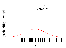
\includegraphics[width=0.5\columnwidth]{./images/particle_filter/gaussian_approximation_by_sampling.pdf}
        \end{center}
        
        \begin{equation*}
            x \leftarrow \frac{1}{2} \sum_{i=1}^{12} \text{rand}(-\sigma, \sigma)
        \end{equation*}
    \end{itemize}

    ¿Cómo samplear utilizando otra distribución?

    \note{Técnica de rejection sampling. No sé utiliza en particle filter porque es una técnica muy ineficiente.}

    \note{Técnica Importance Sampling Principle}

\end{frame}
    


\begin{frame}
    \frametitle{Principio de muestreo de importancia}
    \begin{itemize}
        \item Podemos usar una distribución diferente $\pi$ para generar muestras de $f$
        \item Considere las ``diferencias entre $\pi$ y $f$'' usando un peso $w = f(x) / \pi(x)$
        \item Target $f$
        \item Proposal $\pi$
        \item Precondición:
        $f(x) > 0 \implies \pi(x) > 0$
        \begin{center}
        %\includegraphics[width=0.5\textwidth]{importance_sampling.png}
        \end{center}
    \end{itemize}
\end{frame}
    
\begin{frame}
    \frametitle{Particle Filter}
    \begin{itemize}
        \item Recursive Bayes filter
        \item Non-parametric approach
        \item Models the distribution by samples
        \item Prediction: draw from the proposal
        \item Correction: weighting by the ratio of target and proposal
        \item \textbf{The more samples we use, the better is the estimate!}
    \end{itemize}
    \end{frame}
    
    \begin{frame}
    \frametitle{Particle Filter Algorithm}
    \begin{enumerate}
        \item Sample the particles using the proposal distribution
        \[
        x_t^{[i]} \sim \pi(x_t | \ldots)
        \]
        \item Compute the importance weights
        \[
        w_t^{[i]} = \frac{\text{target}(x_t^{[i]})}{\text{proposal}(x_t^{[i]})}
        \]
        \item Resampling: “Replace unlikely samples by more likely ones”
    \end{enumerate}
    \end{frame}
    
    \begin{frame}
    \frametitle{Monte Carlo Localization}
    \begin{itemize}
        \item Each particle is a pose hypothesis
        \item Proposal is the motion model
        \[
        x_t^{[i]} \sim p(x_t \, | \, x_{t-1}, u_t)
        \]
        \item Correction via the observation model
        \[
        w_t^{[i]} = \frac{\text{target}}{\text{proposal}} \propto p(z_t \, | \, x_t, m)
        \]
    \end{itemize}
    \end{frame}
    
    \begin{frame}
    \frametitle{Particle Filter for Localization}
    \begin{algorithmic}[1]
    \State $\bar{\mathcal{X}}_t = \mathcal{X}_t = \emptyset$
    \For{$m = 1$ to $M$}
        \State Sample $x_t^{[m]} \sim p(x_t \, | \, u_t, x_{t-1}^{[m]})$
        \State $w_t^{[m]} = p(z_t \, | \, x_t^{[m]})$
        \State $\bar{\mathcal{X}}_t = \bar{\mathcal{X}}_t + \langle x_t^{[m]}, w_t^{[m]}\rangle$
    \EndFor
    \For{$m = 1$ to $M$}
        \State Draw $i$ with probability $\propto w_t^{[i]}$
        \State Add $x_t^{[i]}$ to $\mathcal{X}_t$
    \EndFor
    \State Return $\mathcal{X}_t$
    \end{algorithmic}
    \end{frame}
    
    \begin{frame}
    \frametitle{Resampling}
    \begin{itemize}
        \item Survival of the fittest: “Replace unlikely samples by more likely ones”
        \item “Trick” to avoid that many samples cover unlikely states
        \item Needed as we have a limited number of samples
    \end{itemize}
    \end{frame}
    
    \begin{frame}
    \frametitle{Resampling Methods}
    \begin{itemize}
        \item Roulette wheel
        \item Binary search (O(n log n))
        \item Stochastic universal sampling (Low variance, O(n))
    \end{itemize}
    \end{frame}
    
    \begin{frame}
    \frametitle{Low Variance Resampling}
    \begin{algorithmic}[1]
    \State $\bar{\mathcal{X}}_t = \emptyset$
    \State $r = \text{rand}(0; M^{-1})$
    \State $c = w_t^{[1]}$
    \State $i = 1$
    \For{$m = 1$ to $M$}
        \State $U = r + (m - 1) \cdot M^{-1}$
        \While{$U > c$}
            \State $i = i + 1$
            \State $c = c + w_t^{[i]}$
        \EndWhile
        \State Add $x_t^{[i]}$ to $\bar{\mathcal{X}}_t$
    \EndFor
    \State Return $\bar{\mathcal{X}}_t$
    \end{algorithmic}
    \end{frame}
    
    \begin{frame}
    \frametitle{Summary – Particle Filters}
    \begin{itemize}
        \item Particle filters are non-parametric, recursive Bayes filters
        \item Posterior is represented by a set of weighted samples
        \item Not limited to Gaussians
        \item Proposal to draw new samples
        \item Weight to account for the differences between the proposal and the target
        \item Work well in low-dimensional spaces
    \end{itemize}
    \end{frame}
    
    \begin{frame}
    \frametitle{Summary – PF Localization}
    \begin{itemize}
        \item Particles are propagated according to the motion model
        \item They are weighted according to the likelihood of the observation
        \item Called: Monte-Carlo localization (MCL)
        \item MCL is the gold standard for mobile robot localization today
    \end{itemize}
    \end{frame}

\begin{frame}
    \frametitle{Material para Particle Filter}
    
    \begin{itemize}
        \item Información extraída de Vídeo de Cyrill Stachniss https://youtu.be/MsYlueVDLI0
        \item https://rse-lab.cs.washington.edu/projects/mcl/
        \item http://ais.informatik.uni-freiburg.de/teaching/ws12/mapping/pdf/slam09-particle-filter.pdf
    \end{itemize}
   
\end{frame}


\begin{frame}
    \frametitle{TODO}
    \note{Información extraída de Vídeo de Cyrill Stachniss https://youtu.be/MsYlueVDLI0}
    \note{https://rse-lab.cs.washington.edu/projects/mcl/}
    
    \TODO{UTILIZAR LAS SLIDES DEL SEMINARIO}
    
    
\end{frame}


    
